%%%%%%%%%%%%%%%%%%%%%%%%%%%%%%%%%%%%%%%%%%%%%%%%%%%%%%%%%%
%%                                                      %% 
%%      Crowdmark LaTeX Exam Template v0.1              %%
%%                2013-09-20                            %%
%%                                                      %%
%%           Comments or Suggestions?                   %%
%%          email: info@crowdmark.com                   %% 
%%%%%%%%%%%%%%%%%%%%%%%%%%%%%%%%%%%%%%%%%%%%%%%%%%%%%%%%%%

\documentclass[14pt, oneside]{memoir}
\pagestyle{plain}

\usepackage{array, amssymb}
\extrarowheight=5pt
\voffset=-20pt
\textheight=9.5in
%\topmargin=2in
\usepackage{mathtools}
%\usepackage{amsthm}
\usepackage{xcolor}
\usepackage{enumitem}
\newcommand{\erf}{\operatorname{erf}}
\usepackage{graphicx}

\parindent=0pt
\begin{document}


{\textbf{ECO 209 Test 3}}
\vskip 10pt

2025-03-05
\vskip 30pt

\begin{tabular}[t]{l}
%\hline
\hphantom{Last name Last nameLast nameLast name}\\[-15pt]
Last name:  \dotfill  \\
\vspace{0.2cm}

First name: \dotfill  \\

\vspace{0.2cm}
Student ID: \dotfill
%\hline
 \end{tabular}

	\begin{center}
	\fbox{\fbox{\parbox{5.5in}{\centering
				Instructions:
				\begin{enumerate}
					
					\item Read each question carefully before attempting to answer.
					\item Write legibly and preferably in pen.
					\item Explain all of your answers. Show all necessary steps. Be concise.
					\item Make all extra assumptions that you consider necessary but make sure to state them clearly.
					\item Make sure to label all your diagrams appropriately.
					\item You have to hand in the exam sheet. % and any booklets (if any). Please insert additional booklets inside the first booklet before you hand them in.
					%\item If you are using extra booklets, make sure to write your name on each of your books and indicate the order of the booklets (e.g., label them 1 of 2, and 2 of 2).
					\item DO NOT turn this page until instructed.
				\end{enumerate}
				
				
				
				
				Time: 100 minutes
				
				Total Score: 10+15+15+25+15+10 = 90 points; Pages: 18
				
				ONLY Non-Programmable Calculators is ALLOWED
	}}}
\end{center}

\quad
\newpage


\begin{enumerate}[label=\textbf{\arabic*.}, itemsep=15pt]

\item \textbf{(10  pts)}\label{P1}   The quantity equation states that
\[M_t V_t = P_t Y_t\]


\begin{enumerate}[label=(\alph*)]
	\item \textbf{(3 pts)} 	What assumptions about $M_t$, $V_t$, and $Y_t$ are necessary for the \textit{quantity theory of money} to consider the money supply as the key determinant of the price level in the long run?
	
	\vspace{10cm}
	\item \textbf{(2 pts)} Show that the inflation rate, $\pi$, is a function of \textit{only} the growth rates of money supply ($g_M$) and output ($g_Y$). State all the necessary assumptions. 
	
	\clearpage
	%	
	\item \textbf{(2 pts)} As part of the central bank's policy mandate, the central bank aims to maintain an inflation rate of zero percent. Based on the result from part (b), what should the central bank set as the growth rate of the money supply to achieve this goal?
	%growth rate of money supply $g_M$ to the growth rate of output $g_Y$
	
	\vspace{6cm}
	\item \textbf{(3 pts)} In the real world, what challenges might the central bank encounter when implementing the policy you answered in part (c)?
	
\end{enumerate}


\vfill

\newpage
\textbf{Solution}
\begin{enumerate}[label=(\alph*)]
	\item 	
	$M_t$ is controlled by the central bank and is exgenously given 
	
	$V_t$ is constant in the long run
	
	$Y_t$ does not affected by the money market and is determined by only the real variables, according to the classical dichotomy 
	
	Thus, $P_t$ is determined by the $M_t$ only
	
	\item 
	\[g_m + g_V = g_P + g_Y\]
	Let $g_V = 0$ as it is usually assume to be a constant. Therefore,
	\[g_P = \pi = g_m - g_Y\]
	
	\item The central would want to set $\pi = 0$, which implies $g_m = g_Y$
	
	\item The growth rate of the output is hard to predict. Therefore, the central bank may risk creating a negative inflation rate (i.e., deflation) in the short-run. 
	
	\vspace{1cm}
	
	
\end{enumerate}

\clearpage


%\begin{center}
%	This page intentionally left blank. Please continue your answer below.
%\end{center}
%\vspace*{\fill}
%\newpage
%\begin{center}
%	This page intentionally left blank. Please continue your answer below.
%\end{center}
%\vspace*{\fill}
%\newpage

\item  \textbf{(15 pts)}\label{P2} This question focuses on the IS model from Chapter 11. In a closed economy, the consumption ($C_t$), investment ($I_t$), and government purchases ($G_t$) are represented by the following equations:
\[C_t = \bar{a}_c \bar{Y}_t\]
\[\frac{I_t}{\bar{Y}_t} = \bar{a}_I  - \bar{b} \left(R_t - \bar{r}\right) + \bar{x} \widetilde{Y_t}\]
\[G_t = \bar{a}_G \bar{Y}_t \]
The $C$ and $G$ equations are the same as in the simple IS model, while the $I$ equation includes an extension $\bar{x}\widetilde{Y}_t$ where $\bar{x} >0$.

\begin{enumerate}[label=(\alph*)]
	\item \textbf{(2 pts)} What type of observation does the term \( \bar{x} \tilde{Y}_t \) in the investment equation represent or aim to capture?
.
	
	\vspace{7cm}
	\item \textbf{(2 pts)} Name two microeconomic theories that provide the microfoundation for the term \( \bar{a}_c \bar{Y}_t \) in the consumption equation.
	
	
	\newpage
	
	\item \textbf{(5 pts)} Derive the IS curve. Must show all the important steps.
	
	\clearpage
	
	\item \textbf{(3 pts)} The economy is facing a recession where $\widetilde{Y} = -5\%$. The government decided to implement a discretionary policy to stabilize the economy, move the short-run output to zero (i.e., $\tilde{Y}_t = 0$). Given that the parameter $\bar{b} = 0.5$, $\bar{x} = 0.4$ and $\bar{r} = 0.05$. Assume the interest rate stay at the long run level, by how much does the government need to change the $\bar{a}_G$ parameter? 
	

	\vspace{10cm}
	\item \textbf{(3 pts)} 	How much does the government need to change the $\bar{a}_G$ if the $\bar{x} = 0.5$? What is the intuition of it? Explain in one to two sentences.
\end{enumerate}

\clearpage
\textbf{Solution}
\begin{enumerate}[label=(\alph*)]
	\item The term captures the observation that more cash flow during an economic boom, leading to increased investment.

	\item  Permanent Income Hypothesis; Life Cycle Hypothesis.
	
	\item 
		\[Y_t = C_t + I_t + G_t \]
		\[Y_t = \bar{a}_c \bar{Y}_t + \bar{a}_I \bar{Y}_t  - \bar{b} \left(R_t - \bar{r}\right) \bar{Y}_t + \bar{x} \widetilde{Y_t} \bar{Y}_t + \bar{a}_G \bar{Y}_t \] 
		\[\frac{Y_t}{\bar{Y}_t}-1 =\widetilde{Y_t} = \bar{a}_c + \bar{a}_I  - \bar{b} \left(R_t - \bar{r}\right)  + \bar{x} \widetilde{Y_t} + \bar{a}_G -1 \] 
		\[\widetilde{Y_t} = \bar{a} - \bar{b} \left(R_t - \bar{r}\right)  + \bar{x} \widetilde{Y_t}   \] 
		\[\widetilde{Y_t} = \left(\frac{1}{1-\bar{x}}\right)\left[\bar{a} - \bar{b} \left(R_t - \bar{r}\right) \right]  \]
	
	
	\item  The government needs to increase $a_G$ by $5\% \times \left(1-0.4\right) = 3\%$

	\item The government needs to increase $a_G$ by $5\% \times \left(1-0.5\right) = 2.5\%$. 
	
	A higher value of \(\bar{x}\) indicates that investment is more sensitive to the output gap. Thus, for a given output gap, a larger \(\bar{x}\) necessitates a more substantial fiscal policy adjustment (i.e., a larger change in \(\bar{a}_G\)) to close the gap. In this case, as \(\bar{x}\) increases from 0.4 to 0.5, the government must reduce \(\bar{a}_G\) by a slightly larger amount to counteract the negative output gap.
	
	(The multiplier story is accepted as well.)
\end{enumerate}

\clearpage

%\newpage
%\begin{center}
%	This page intentionally left blank. Please continue your answer for q.2 below.
%\end{center}
%\vspace*{\fill}

\newpage

\item  \textbf{(15 pts)}\label{P3} You are given the following quarterly GDP data from 2010 to 2013:

\vspace{4mm}

% Table generated by Excel2LaTeX from sheet 'Sheet1'
\begin{table}[htbp]
	\centering
	\begin{tabular}{lcccccccc} \hline \hline
		Time  & 2010Q1 & 2010Q2 & 2010Q3 & 2010Q4 & 2011Q1 & 2011Q2 & 2011Q3 & 2011Q4 \\ 
		GDP   & 4298  & 4321  & 4351  & 4400  & 4433  & 4441  & 4502  & 4538 \\ \hline
		&       &       &       &       &       &       &       &  \\ \hline
		Time  & 2012Q1 & 2012Q2 & 2012Q3 & 2012Q4 & 2013Q1 & 2013Q2 & 2013Q3 & 2013Q4 \\
		GDP   & 4541  & 4555  & 4562  & 4571  & 4612  & 4638  & 4677  & 4726 \\ \hline \hline
	\end{tabular}%
	\label{tab:addlabel}%
\end{table}%


\vspace{4mm}

\begin{enumerate}[label=(\alph*)]
	\item \textbf{(3 pts)} Calculate the 3-quarters Trailing Simple Moving Average (SMA) from 2013Q1 to 2013Q3. If applicable, keep two digits after the decimal point.
	\clearpage
	\item \textbf{(4 pts)} Use the SMA as the trend and calculate short run output (i.e., percentage derivation from the potential output) for \textit{2013Q1 to 2013Q3}. 
	
	If applicable, keep four digits after the decimal point or two digits if the result is expressed in percentage.
	\vspace{8cm}
	\item \textbf{(5 pts)} Following Hamilton's approach, the estimated regression model is given by:
	\[
	y_{t+8} = 118.47 + 0.55 y_{t} + 0.05 y_{t-1} + 0.15 y_{t-2} + 0.27 y_{t-3} + \nu_{t+8}
	\]
	Using the estimated model, calculate the trend and cyclical component (as a percentage deviation from the trend) of Real GDP for Canada for \textit{2013Q1 to 2013Q2}.
	\clearpage
	\vspace*{10cm}
	\item \textbf{(4 pts)} Provide two reasons why the Hamilton Filter is better than simple moving average.
\end{enumerate}
\newpage

\textbf{Solution}
\begin{enumerate}[label=(\alph*)]
	\item \textbf{(3 pts)} 
	
	\[SMA_{13,Q1} = \frac{4562+4571+4612}{3} = 4581.67\]
	
	\[SMA_{13,Q2} = \frac{4571+4612+4638}{3} =  4607 \]
	
	\[SMA_{13,Q3} = \frac{4612+4638+4677}{3} =4642.33\]
	
	\item \textbf{(4 pts)} 
	
	\[\tilde{Y}_{13,Q1} = \frac{4612}{4581.67} - 1 = 0.0066	\]
	
	\[\tilde{Y}_{13,Q2} = \frac{4638}{4607} - 1 = 0.0067	\]
	
	\[\tilde{Y}_{13,Q3} = \frac{4677}{4642.33} - 1 = 0.0075	\]
	
	\item \textbf{(5 pts)}
	The potential output/trend are:
	\[
	118.47 + 0.55 \times 4433 + 0.05 \times 4400 + 0.15 \times 4351 + 0.27 \times 4321 = 4595.94
	\]
	\[
	118.47 + 0.55\times 4441 + 0.05 \times 4433 + 0.15 \times 4400 + 0.27 \times 4351 = 4617.44
	\]

	Cyclical component:
	
	\[\tilde{Y}_{13,Q1} = \frac{4612}{4595.94} - 1 = 0.0035\]
	
	\[\tilde{Y}_{13,Q2} = \frac{4638}{4617.44} - 1 = 0.0045\]
	\clearpage
	\item \textbf{(4 pts)} 
	\begin{itemize}
		\item The Hamilton filter is based on regression approach, which is more theoretically grounded than SMA.
		\item It allows to include structural breaks and changes in the data, offering better adaptability in different economic environments
		\item Better forecasting ability with the Hamilton Filter.
		\item Preserves Basic Time Series Properties
	\end{itemize}
\end{enumerate}

\newpage

\item  \textbf{(25 pts)}\label{P4} The IS curve show the relationship between the real interest rate (\( R_t \)) and short-run output (\( \tilde{Y}_t \)). A simplified form of the IS curve is given by:

\[
\tilde{Y}_t = \bar{a} - \bar{b} (R_t - \bar{r})
\]

where \( \tilde{Y}_t \) is the short-run output, \( R_t \) is the real interest rate, \( \bar{r} \) is the marginal product of capital,  \( \bar{a} \) captures aggregate demand and \( \bar{b} \) represents the sensitivity of investment to changes in the real interest rate.

Assume the economy starts at its long-run equilibrium position.

\begin{enumerate}
	\item \textbf{(3 pts)} Explain the economic intuition behind the downward slope of the IS curve. Why does a decrease in the real interest rate (\( R_t \)) lead to an increase in short-run output (\( \tilde{Y}_t \))?
	
	\clearpage
	
	\item \textbf{(5 pts)} Suppose the government increases its spending. Using the IS curve equation, explain how this policy affects short run output in the short run given the interest rate is fixed. Illustrate this by drawing a graph with the interest rate (\( R_t \)) on the Y-axis and short-run output (\( \tilde{Y}_t \)) on the X-axis. Clearly indicate the initial equilibrium and the new equilibrium after the shock.
	
	\vspace{10cm}
	\item \textbf{(3 pts)} Why might the government choose to increase its spending in the real world? Provide two reasons.
	
	\clearpage
	\item \textbf{(5 pts)} How does an increase in \( \bar{b} \) affect the slope of the IS curve? Illustrate this by drawing two IS curves on a graph, labeling the one with a higher \( \bar{b} \) as \( IS' \). The graph should have the interest rate (\( R_t \)) on the Y-axis and short-run output (\( \tilde{Y}_t \)) on the X-axis.
	
	\vspace{10cm}
	\item \textbf{(2 pts)} How does an increase in government spending impact short-run output when the \( \bar{b} \) parameter is larger?
	
	\clearpage
	\item \textbf{(5 pts)} (Separate from part b)) A tornado destroyed half of the capital in the economy. Besides lowering the potential output and actual output, it also increases the Marginal product of capital. Illustrate this by drawing a graph with the interest rate (\( R_t \)) on the Y-axis and short-run output (\( \tilde{Y}_t \)) on the X-axis. Label the initial point as $A$ and the new point after the shock as $B$. Label the initial IS curve as $IS$ and the new IS curve as $IS'$. 
	
	\vspace{10cm}
	\item \textbf{(2 pts)} How would the increase in \( MPK \) impact short-run output in this scenario if the interest rate is kept at initial level? Explain in 1-3 sentences.
	
\end{enumerate}

\clearpage
\textbf{Solution}

\begin{enumerate}
	\item 
	The IS curve shows that a decrease in the real interest rate reduces the benefit from saving (or lower the cost of borrowing), which induce more investment. This higher aggregate demand increases short-run output \(\tilde{Y}_t\). 
	
	\bigskip
	
	\item 
	An increase in government spending raises aggregate demand, thereby increasing \(\bar{a}\) in the IS curve equation:
	\[
	\tilde{Y}_t = \bar{a} - \bar{b} (R_t - \bar{r}).
	\]
	This shifts the IS curve to the right. With the real interest rate \(R_t\) fixed, short-run output rises. 
	
	\begin{figure}[htbp!]
		\centering
		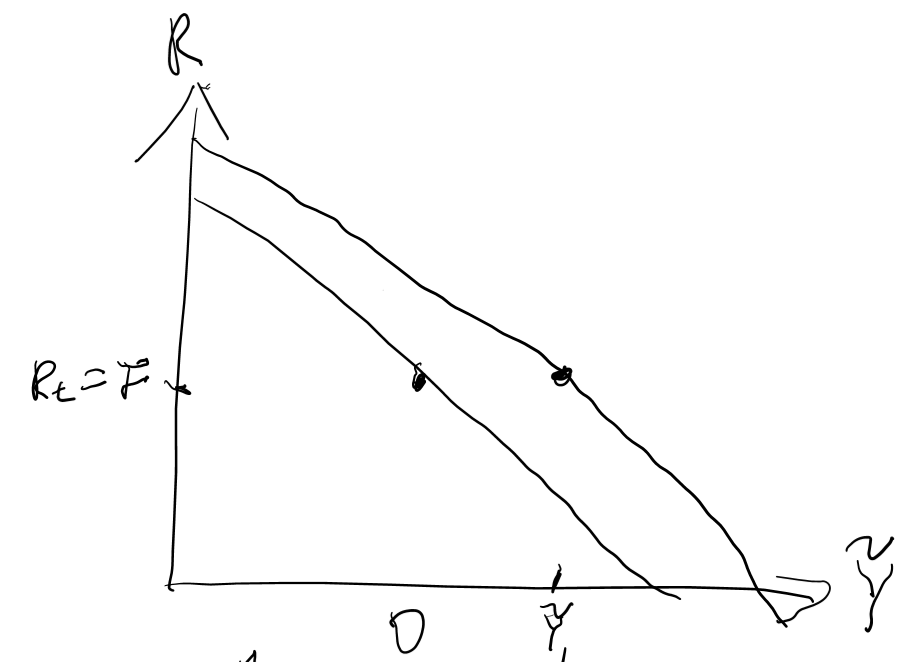
\includegraphics[width=0.7\linewidth]{figure/q4b}
	\end{figure}
	
	\bigskip
	
	\item 
	Policymakers may increase government spending to:
	\begin{enumerate}[label=(\arabic*)]
		\item Stimulate aggregate demand during recessions
		\item Reduce unemployment by injecting additional spending into the economy.
		\item Election cycle.
	\end{enumerate}
	
	\bigskip
	\clearpage
	\item 
	A higher \(\bar{b}\) means investment is more sensitive to changes in the real interest rate, which steepens the IS curve. 
	
	\bigskip
	
	\item 
	With a larger \(\bar{b}\), the IS curve becomes steeper, meaning that short-run output is more sensitive to changes in the real interest rate. Consequently, if \(\bar{a}\) increases by the same amount in both cases, the impact on short-run output remains consistent, regardless of the increase in \(\bar{b}\).
	
	\begin{figure}[htbp!]
		\centering
		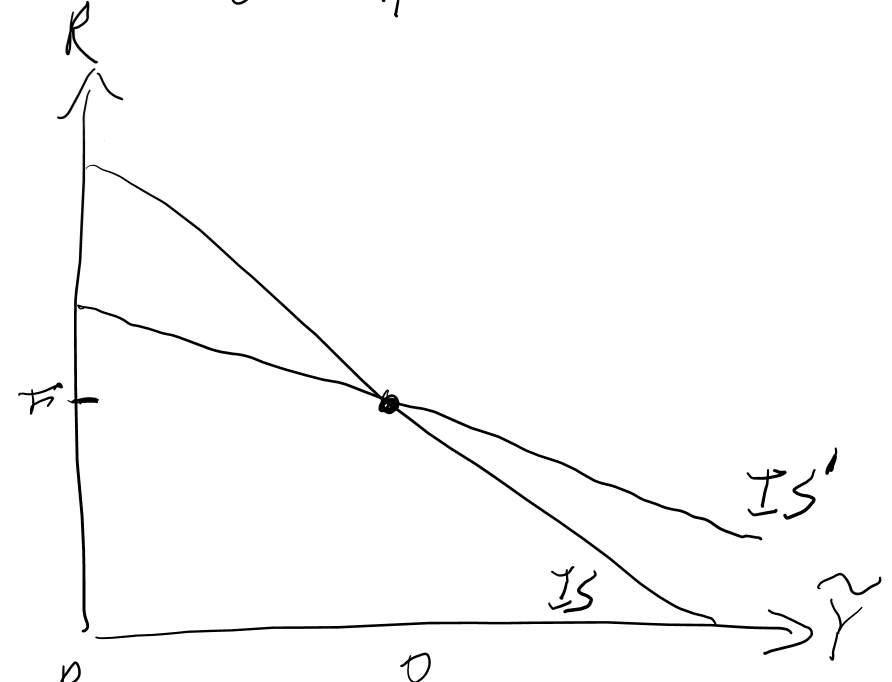
\includegraphics[width=0.7\linewidth]{figure/q4d}
	\end{figure}
	
	
	\bigskip
	
	\item
	The question didn't specific if the point B should be representing the long-run or short-run. Both point B or B' on the graph would be accepted.
	\clearpage
	\begin{figure}[htbp!]
		\centering
		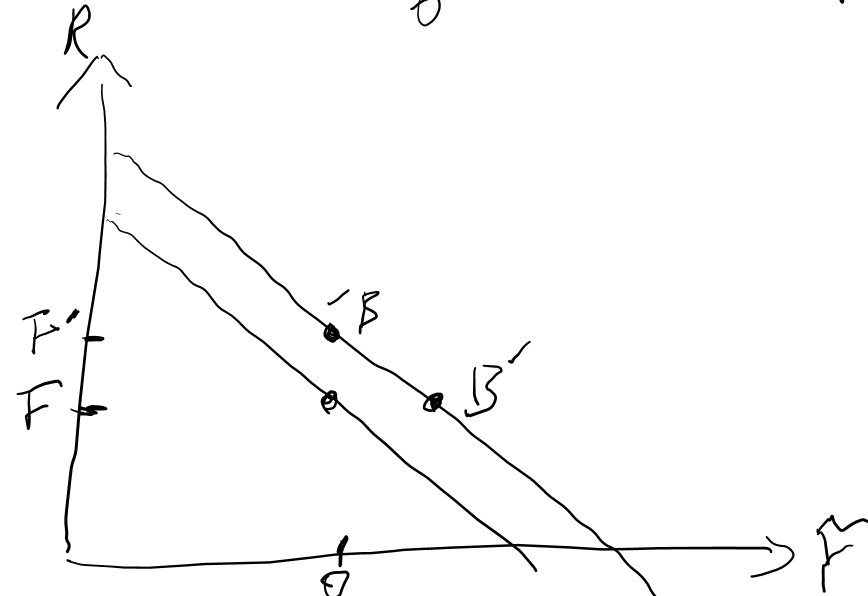
\includegraphics[width=0.7\linewidth]{figure/q4f}
	\end{figure}
	
	
	\bigskip
	
	\item Effect of Increased MPK on Short-Run Output (2 pts)  
	\medskip
	
	If the interest rate is held constant, an increase in MPK raises the productivity of the remaining capital, which tends to increase short-run output (i.e., when MPK>R, firms invest). 
	
\end{enumerate}




\clearpage
\item  \textbf{(15 pts)}\label{P5} Impulse Cafe is considering purchasing a second espresso machine by taking out a loan of \$21,000 from the bank at an 6\% interest rate. The corporate tax rate is 15\%. Currently, the cafe operates with only one espresso machine. Acquiring an additional machine would enable the cafe to produce 1,500 extra shots of espresso, with each shot selling for \$3. The depreciation rate of the espresso machine is 3\%.

\begin{enumerate}[label=(\alph*)]	
	\item \textbf{(3 pts)} Should Impulse Cafe invest in the new espresso machine? Provide an explanation for your reasoning.
	\vspace{7cm}
	\item \textbf{(4 pts)} Now, assume Impulse Cafe is considering acquiring additional espresso machines, where each successive espresso machine is less productive than the previous one. The MPK of the \( k \)th espresso machine is given by \( \frac{1500}{K} \). Given the same prices and depreciation rate as in part (a), how many espresso machine should Impulse Cafe purchase to maximize its profit?
	
	\clearpage
	\vspace*{4cm}
	\item \textbf{(4 pts)} How many machines should Impulse Cafe operate if the government increases the corporate tax rate to 30\%?
	\vspace{7cm}
	\item \textbf{(4 pts)} After raising the corporate tax rate to 30\%, the government allocates a portion of the collected tax revenue to subsidize new equipment purchases as an investment incentive. How many machines should Impulse Cafe operate if the purchasing price is reduced to \$16,000?
\end{enumerate}

\clearpage

\textbf{Solution}
\begin{enumerate}[label=(\alph*)]
	\item The MPK in dollar term is $1500\times \$3 = \$4500$. Using the formula,
	\[\frac{MPK}{p_K} = \left(\frac{1}{1-\tau}\right)\left[R+\delta -\frac{\Delta p_K}{p_K}\right]\]
	\[\frac{4500}{21000}= 0.21 > \left(\frac{1}{1-0.15}\right)\left[0.06+0.03 \right]  = 0.106\]
	As the LHS is greater than the RHS, the Bistro should invest in the new espresso machine
	\item We can sub in $1500/K$ as MPK. 
	\[\frac{1500\times 3}{21000 K} = 0.106 \implies K=2.02\]
	\item 
	\[\frac{1500\times 3}{21000 K} = \left(\frac{1}{1-0.30}\right)\left[0.06+0.03 \right]= 0.1286  \implies K=1.66\]
	\item Now the price of the capital is lowered to 16,000
	
	\[\frac{1500\times 3}{16000 K} = 0.1286  \implies K=2.19\]
\end{enumerate}



%\newpage
%\begin{center}
%	This page intentionally left blank. Please continue your answer below.
%\end{center}
%\vspace*{\fill}
%
%\newpage
%\begin{center}
%	This page intentionally left blank. Please continue your answer below.
%\end{center}
%\vspace*{\fill}

\newpage
%
\item  \textbf{(10 pts)}\label{P6} 
Suppose Country A has a Phillips curve that is relatively steep compared to Country B, answer the following:

\begin{enumerate}[label=(\alph*)]
	\item \textbf{(5 pts)} How would the two countries respond to the same percentage fall in output? Demonstrate it graphically with the two Phillips curves plotted on a graph. Label all axes and points of interest.
	
%	\item[] Country A will have  faster fall in rate of inflation. 
%	
%	\begin{figure}[htbp!]
%		\centering
%		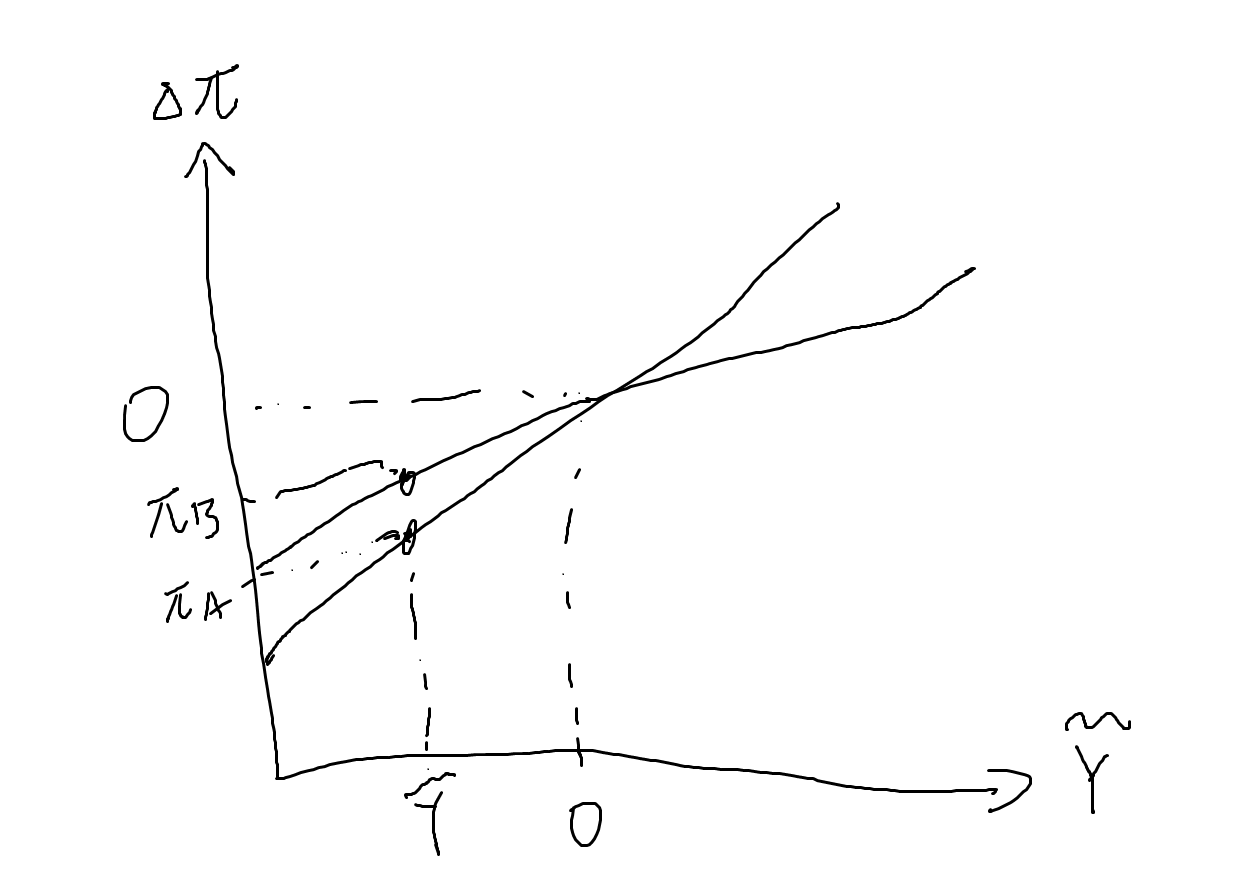
\includegraphics[width=0.7\linewidth]{figure/q6}
%	\end{figure}
		
	\vspace{11cm}
	\item \textbf{(3 pts)} What are some factors that might influence the slope of the Phillips curve?
%	\item[] People aren’t used to seeing inflation change: maybe inflation has been stable for years, so they don’t think about it much. Alternatively, government rules or strong monopoly or union power could make it difficult to change prices in the dashed economy.
	
	\clearpage
	\item \textbf{(2 pts)} Suppose the economy experiences a significant and unexpected surge in productivity growth that lasts for a decade due to innovations in air fryers, which allow company to make potato chips at large scale. Policymakers are slow to respond to this shock, causing actual output to exceed potential output. How does this impact short-run output and the inflation rate?
\end{enumerate}

\clearpage
\textbf{Solution}
\begin{enumerate}[label=(\alph*)]
	\item \textbf{(5 pts)}  Country A will have faster fall in rate of inflation. 
		\begin{figure}[htbp!]
			\centering
			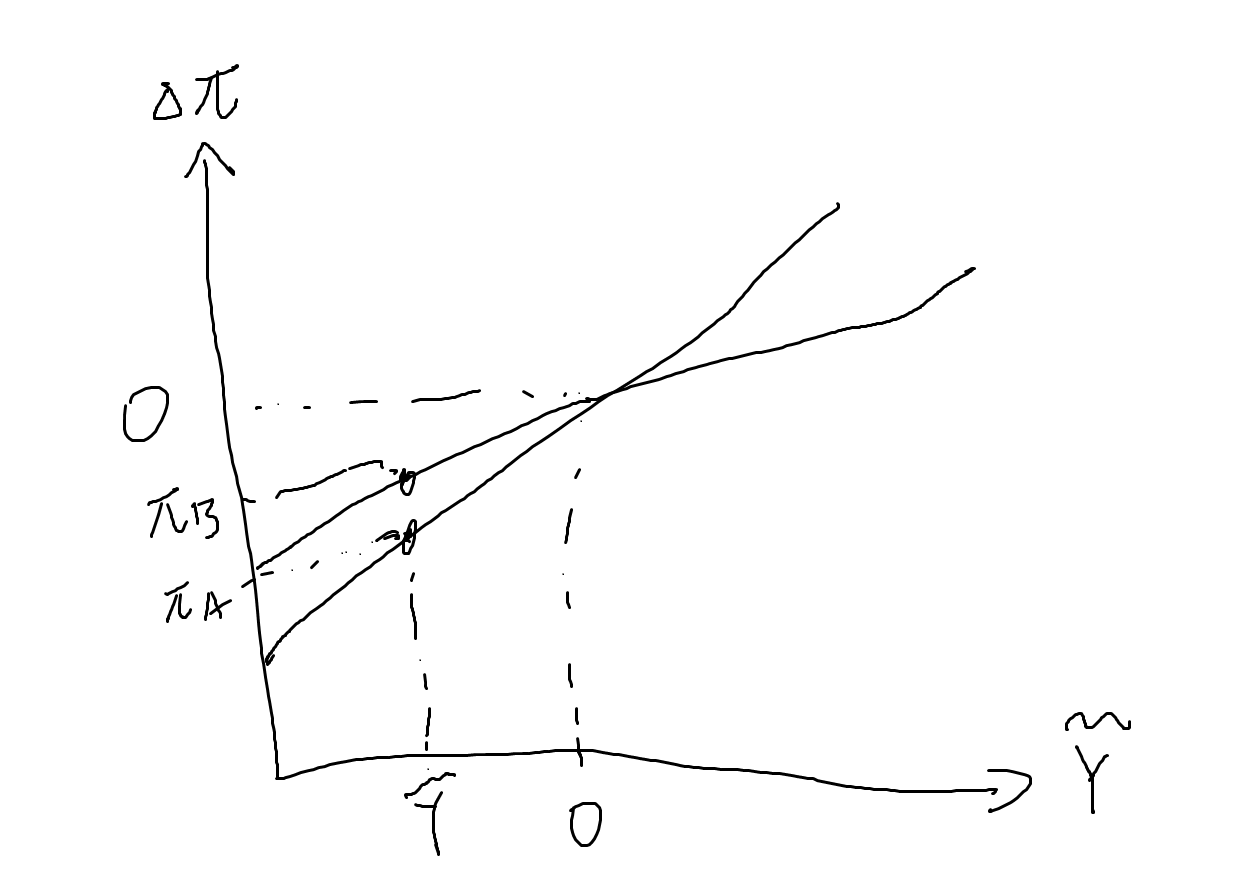
\includegraphics[width=0.7\linewidth]{figure/q6}
		\end{figure}
	
	\item \textbf{(3 pts)} The Phillips curve is upward sloping because during an economic boom, higher demand forces firms to produce above their potential, leading to rising prices. Consequently, any factor that influences this pricing behavior will affect the slope of the Phillips curve.
	
	*Any other plausible factor should be considered a valid answer.
	
	\bigskip
		
	\clearpage
	\item \textbf{(2 pts)} 	
		A significant and unexpected surge in productivity raises potential output. However, if policymakers delay their response, actual output will temporarily exceed potential output, pushing the economy up along the Phillips curve. As a result, the inflation rate will be higher than zero (or the long-run inflation target).
\end{enumerate}


%\newpage
%\begin{center}
%	This page intentionally left blank. Please continue your answer below.
%\end{center}
%\vspace*{\fill}

\newpage
\begin{center}
	This page intentionally left blank. Please continue your answer below.
\end{center}
\vspace*{\fill}
%
%\newpage
%\begin{center}
%	This page intentionally left blank. Please continue your answer below.
%\end{center}
\vspace*{\fill}

\centering{-- The End -- }
\end{enumerate}
  \end{document}
